\documentclass{acm_proc_article-sp}
\usepackage{wrapfig}
\usepackage{tikz, alex, url, mu}
\usetikzlibrary{arrows,shapes,snakes,automata,backgrounds,petri}
\tikzset{>=stealth}

\title{Quilting for Distributed Machine Learning System}

\author{Mu Li \\ CMU CSD \and Jinliang Wei\\ CMU CSD}

\begin{document}
\maketitle

\begin{abstract}
  Distributed machine learning applications produces a huge amount of network
  traffic. However, network bandwidth is one of the most scarce resources in
  datacenters.  In this paper we proposal QuiltDB, a distributed database
  execution engine optimized for network topology. QuiltDB trades off latency
  for high bandwidth. It executes in a discrete streaming fashion and allows
  users to specify desirable network topologies. We evaluate this system on
  several machine learning applications with real datasets\footnote{C++ codes
    are available at \url{https://github.com/jinliangwei/quiltdb/}}.
\end{abstract}

\section{Introduction}

In distributed machine learning applications, data,  as well as computation, are
partitioned into hundreds or  thousands of machines. Those
worker machines compute local results based on their own part of data. Global solutions
are then obtained via synchronization.

Machine synchronization, including data communication and waiting, is typically
the most expensive operation, because of limited network bandwidth and highly
variant machine performances. Recently, asynchronous communication is proposed
to hide the synchronization cost, however, those works assume the network has
uniform point-to-point bandwidth.

However, the real data datacenter network usually has specially topology. For
example, machines are grouped by ranks, and those ranks are then connected by
several layers of switchers. It thus forms a (multi-)tree like
topology. Machines within a rack has much larger bandwidth than crossing racks.

It is necessary to consider the network topology, because of the huge amount of
data communication volume and iterative nature of  machine learning
applications. In addition, if the communication forms a simple pattern, such as
a ring or a start, then it is much easier to improve the machine network
according this to pattern than improve the overall point-to-point bandwidth.

On this paper, we propose a database execute engine, QuiltDB, which mapping
machine learning applications into network topologies. Key features of this
system includes,

\begin{itemize*}
\item Grid data partition. Traditional databases uses either vertical or
  horizontal partition. However, a grid partition could reduce the network
  traffic volume if the training data is near square, namely the number of
  instances and features are on the same scale.
\item Model machine learning applications using the
  primal-dual approach. The primal-dual decomposition fits into the grid
  partition in nature, where the primal variables are shared horizontally, while
  the dual variables are communicated vertically.
\item Allow use-defined network topology.
\item A discrete streaming system.
\end{itemize*}

\section{Network Topologies}
\label{sec:network-topologies}

Several network topologies have been proposed by HPC community, including grid,
hyper-cube, buffer-fly, etc. Algorithms are then mapped into network topology to
maximize the communication efficiency. On the other hand, cloud computing
typically adopts
tree-like structures, which aims to approximate an uniform all-to-all connection
and provide fault tolerance and elastic scalability.

\subsection{Grid Communication}

Grid is the one of the simplest communication pattern, which is shown in
Figure~\ref{fig:grid2}. Machines are connected both vertically and
horizontally. Each machine only communicates with its 4 neighbors. Its
restricted connections make it comparable cheap to build the physical
network. It also relieves switchers' burden on the cloud computing setting.
However, if the two machines are far away, then the network delay between these
two is also large.

\begin{figure}[th!]
  \centering
  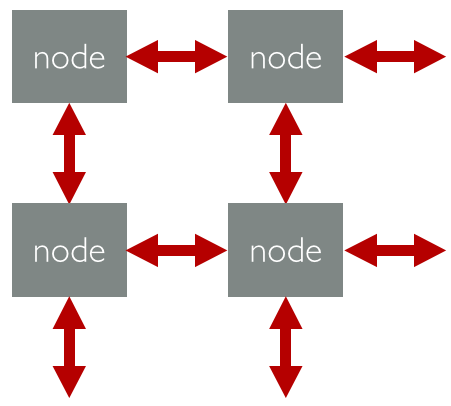
\includegraphics[width=.25\textwidth]{fig/grid}
  \caption{Grid communication}
  \label{fig:grid2}
\end{figure}

\subsection{Two-layer Network}

The grid communication is somewhat too restrictive. Nowadays machines within a
datacenter are typically first connected by top-rack switchers. Due to the high
bandwidth in a switcher, machines in the same rack usually have decent
point-to-point bandwidth. Therefore we may use more flexible within rack
communication pattern. Figure~\ref{fig:rack} shows a simple example, where
machines only talk to the others in the neighbor rack, while any two machines
within the same rack could communicate.
\begin{figure}[th!]
  \centering
  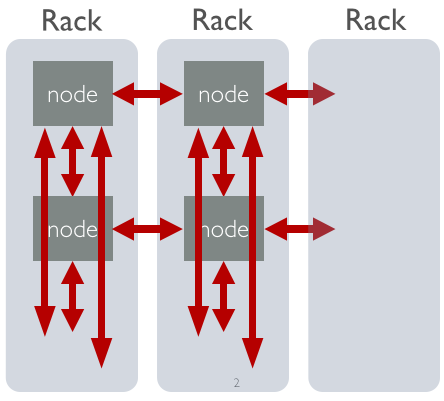
\includegraphics[width=.25\textwidth]{fig/rack}
  \caption{More flexible within rack communication.}
  \label{fig:rack}
\end{figure}

\section{Machine Learning Applications}

On this section, we describe several machine learning applications which fits
into the communication pattern we discussed on Section
\ref{sec:network-topologies}.

\subsection{Data Partition}

On a typical distributed machine learning application, both data and shared
parameters are partitioned into a group of machines.
Different partitioning scheme requires different amount of data to be
communicated. For example, consider the following iterative matrix
multiplications, which is a typical machine learning workload:
\begin{align*}
w &= X u \\
u &= X^T w,
\end{align*}
where $X$ is a gigantic data matrix and $u$ and $w$ are two vectors.

Given a $n$-by-$m$ matrix $X$, we want to divide the matrix into $p$ machines
while minimizing the amount of data to be communicated in each iteration.

If we cut the matrix into $a$ rows and $b$ columns, then the minimal data
communication is

\begin{equation}
  r  am +  c bn
  \label{eq:total-traffic}
\end{equation}
where $r,c \in [0,1]$ are coefficient depending on the sparsity of the
matrix. They should be a function as $a$ and $b$, but now we consider it as a
constant to simply the calculation.

Note that $ab=p$, then (\ref{eq:total-traffic}) get minimize value when
$a = \rbr{ \frac{cn}{rm} }^{\frac{1}{2}}\sqrt{p}$. That is, if $cn \gg rm$, we
should choose partition scheme 1, if $rm \gg cn$, we should use scheme 2, while
if $rm \approx cn$, the even partition scheme 3 is a better choice.

\begin{figure}[th!]
  \centering
\begin{tikzpicture}[scale=.5]
  \draw [fill=set12!60](0,0) rectangle (4,1)
  rectangle (0,2) rectangle (4,3) rectangle (0,4);
  \draw[xshift=6cm, fill=set11!60] (0,0) rectangle (1,4) rectangle (2,0) rectangle (3,4)
  rectangle (4,0);
  \draw[xshift=12cm, fill=set13!60] (0,0) rectangle (2,2) rectangle (0,4);
  \draw[xshift=14cm, fill=set13!60] (0,0) rectangle (2,2) rectangle (0,4);
\end{tikzpicture}
  \caption{partition scheme 1 to 3: $a=4,b=1$, $a=1,b=4$, and $a=2,b=2$}
\end{figure}

\subsection{Pagerank}
\label{sec:pagerank}

Given adjacent matrix $X$, where $X_{ij} = 1 $ if and only if webpage $i$ cites
$j$. Denote by $D=\textrm{diag}{\sum_i X_{i1}, \ldots, \sum_{i=1} X_{in}}$ the diagnal
adjacent matrix, then pagerank can be solved by.
\begin{equation}
  w = \alpha X^T D^{-1} w + (1-\alpha)\frac{1}{n}
\end{equation}

\begin{figure}[th!]
  \centering
  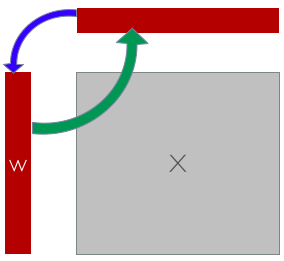
\includegraphics[width=.25\textwidth]{fig/pr}
  \caption{Pagerank}
  \label{fig:pr}
\end{figure}

The workload is summarized in Figure~\ref{fig:pr}. It is convenient to view the
updating as two steps, the
first step compute the new value of $w$, and then update $w$. To extend pagerank
into a distributed algorithm, we consider the grid data partition. Then each
machine also execute the computing and then updating steps. The only difference
is that updating involves network communications. On the example, each rack get
a group of columns of $X$. One particular  machine in the rack gathers the
updates within the rack and then propagates to other racks.

\begin{figure}[th!]
  \centering
  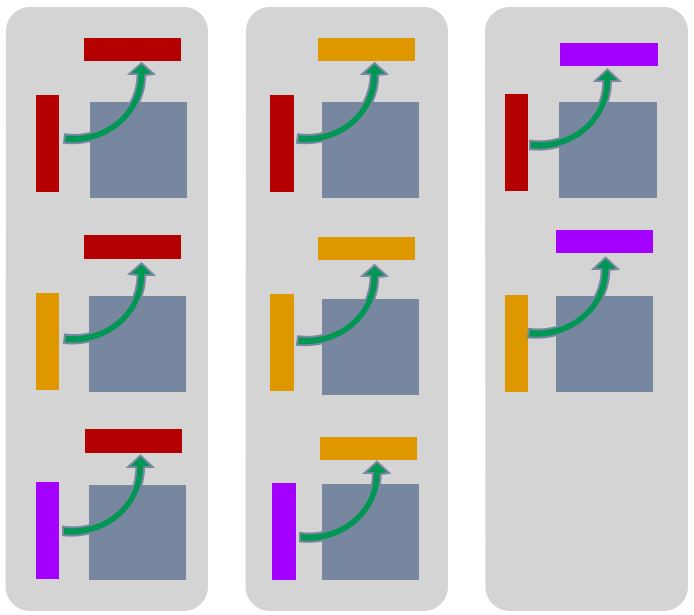
\includegraphics[width=.25\textwidth]{fig/compute}
  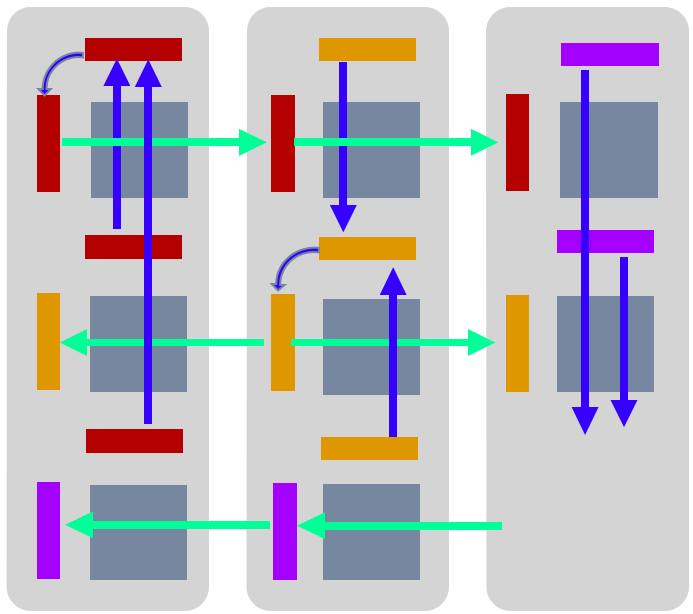
\includegraphics[width=.25\textwidth]{fig/update}
  \caption{Two steps of pagerank: compute and then update}
\end{figure}

\subsection{Loss minimization}

Loss minimization solves the following optimization problem:
\begin{equation}
  \min_w \sum_{i=1}^{n} f(\langle x_i, w\rangle, y_i) + \lambda r(w)
\end{equation}
It fits into our setting by considering the primal-dual view, where $w$ is the primal
variable, while $\partial f(\langle x_i, w\rangle, y_i) x_i$ is the dual. Then
the optimization method computes and updates the prime and dual alternatively.

\section{Programming Model}

QuiltDB provides a distributed in-memory key-value store for accessing shared 
data. Key-value pairs are organized as tables and tables are shared among 
nodes along the same \emph{oplog propagation path}. Updates to shared key-value 
pairs are propagated along \emph{oplog propagation path}s. Typically, a QuiltDB 
process occupies a physical node and it
consists of multiple \emph{logical node}s. Each \emph{logical node} may 
participate in one \emph{oplog propagation path}. That is, a \emph{logical node}
receives updates generated by other nodes along the path and forwards them to 
its downstream node along with its own updates. With multiple \emph{logical 
node}s, a QuiltDB process may participate in multiple \emph{oplog propagation 
path}s. With the help of callback functions (Section~\ref{sec:callback}) 
participating in multiple \emph{oplog propagation path}s
allows a QuiltDB process to act as hub to relay updates along one path to 
another path.

When using QuiltDB, the user needs to configure the network topology 
(\emph{oplog propagation path}s). QuiltDB lets user provide information of 
each \emph{logical node} and configure the network topology by simply choosing 
the proper downstream node for each \emph{logical node}. A \emph{logical node} 
may have at most one downstream node, while it may have many upstream nodes. 
Having multiple upstream nodes allows a single node to aggregate updates from 
multiple sources. Restricting a \emph{logical node} to have only one downstream 
node allows QuiltDB to support cyclic \emph{oplog propagation path}s with simple 
oplog deduplicatoin mechanism (see Section~\ref{sec:cyclic-path}).


\begin{figure}[th!]
\begin{verbatim}
class Table{
  template<typename ValueType>
  ValueType Get(int64_t _key);

  template<typename ValueType>
  void Inc(int64_t _key, ValueType _delta);
};

typedef int (*ValueAddFunc)(uint8_t *v1,
                            const uint8_t *v2,
                            int32_t size);
typedef int (*ValueSubFunc)(uint8_t *v1,
                            const uint8_t *v2,
                            int32_t size);

\end{verbatim}
\caption{Semantics of QuiltDB table APIs and the addition and subtraction
  functions}
\label{fig:table-api}
\end{figure}

\subsection{Key-Value Interface}

As mentioned above, the data stored in QuiltDB are key-value pairs organized 
as tables. Values are treated as byte array internally and values stored in one 
table are required to have the same size. Supporting multiple tables allows 
QuiltDB to support different types of data.

QuiltDB requires the value type to support two operations, \emph{addition} and
\emph{subtraction}. In order to support update aggregation, \emph{addition} must
 be commutative and associative. For numerical types,  the meaning of 
\emph{addition} and \emph{substraction} are straightforward. The interface of 
QuiltDB tables and the semantics of addition and subtractions are shown in
Figure~\ref{fig:table-api}.

The only write operation supported by the key-value storage is INC which takes
in a delta and apply the delta to a value via \emph{addition}.

\subsection{Callback Functions}
\label{sec:callback}

In most cases, when updates from other nodes are received, they are applied to
local copy of shared data and forwarded to downstream node silently.
However, there are applications that need to be notified upon receiving updates
to perform some special procedure, such as relaying the updates received from
one path to another. For this special case, QuiltDB allows aplication to
register a callback per table which is executed upon the receipt of updates. As
said in Section~\ref{sec:pagerank}, the callback function is essential to
propagate updates to other ranks.

Application may set proper flags on a table to let QuiltDB perform any
combination of the three actions on received updates: 1) apply them on local
copy, 2)forward them to downstream node and 3) execute user callback.

\section{Implementation}
In this section, we discuss our system implementation along with techniques to
minimize communication cost.

\begin{figure}[th!]
  \centering
  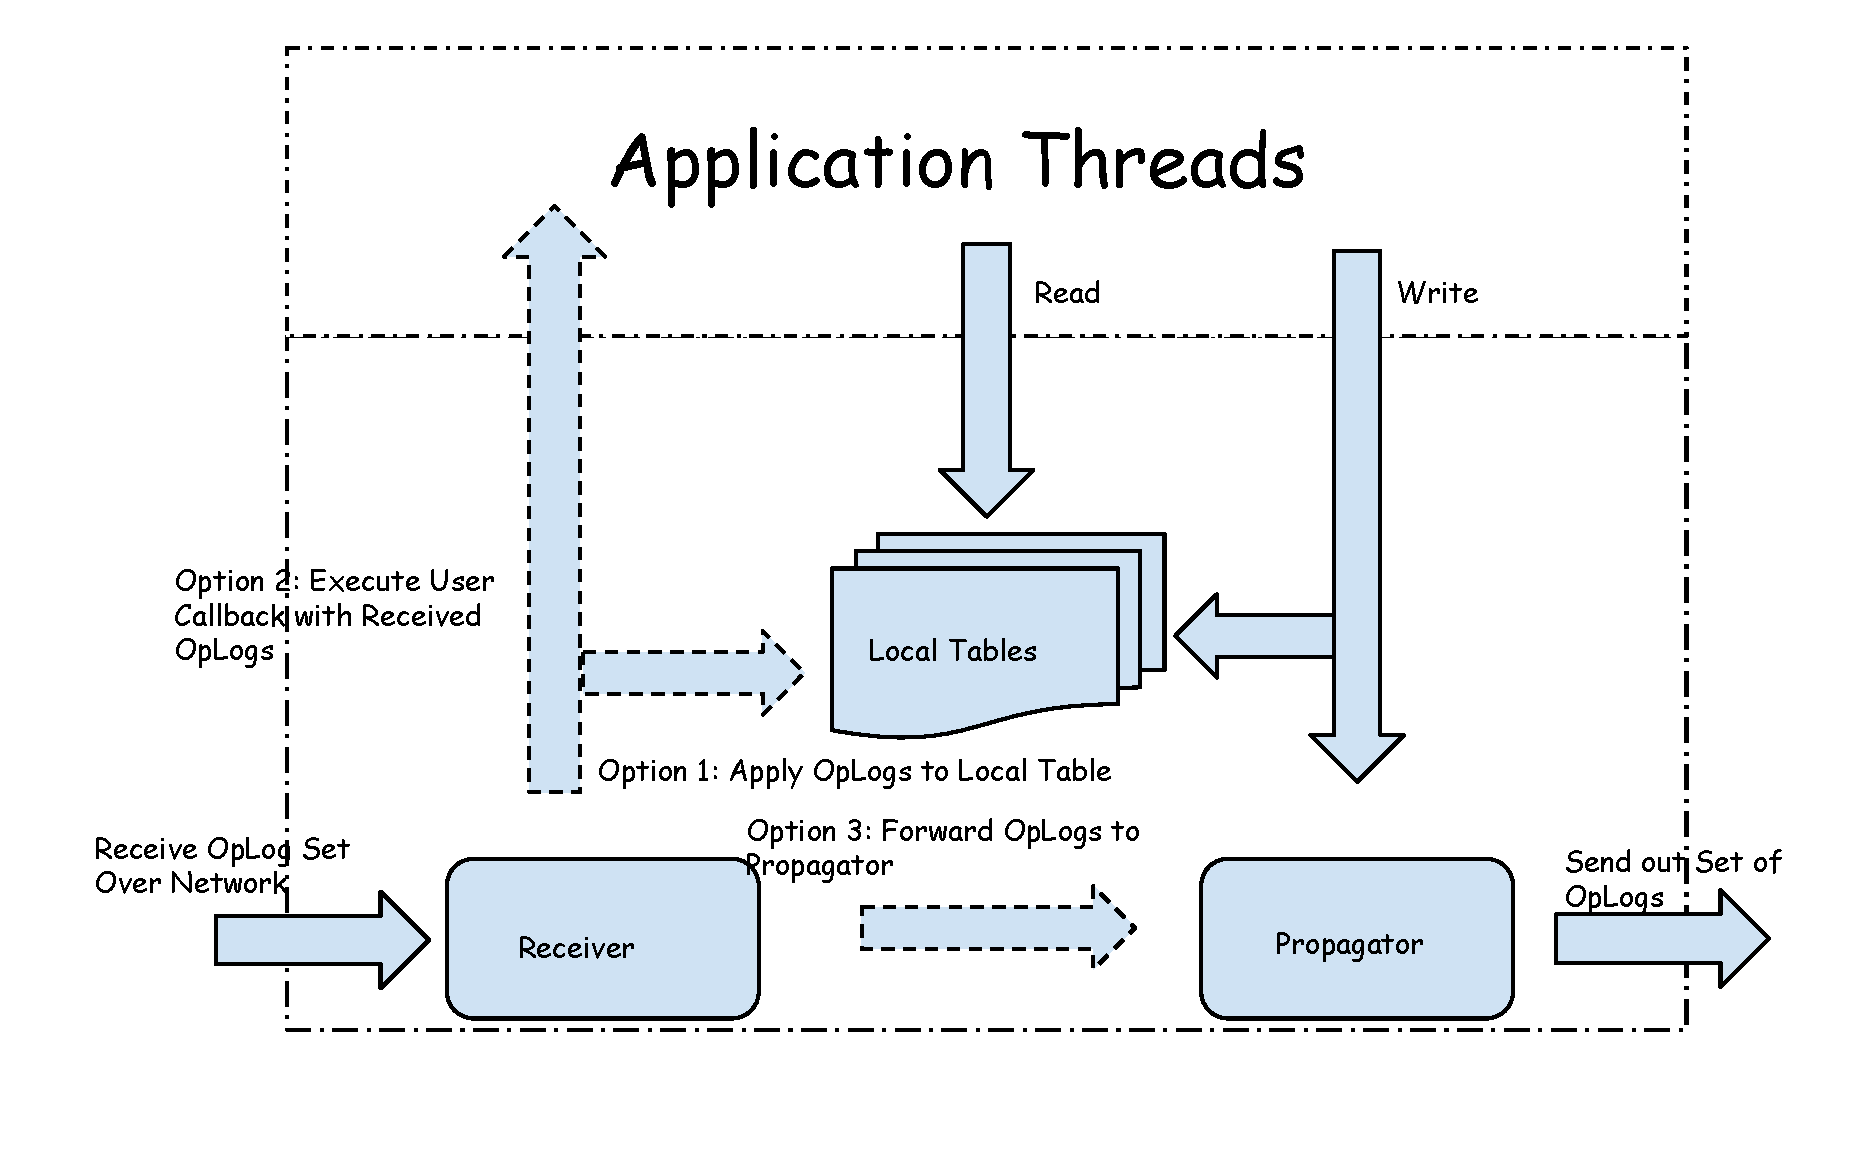
\includegraphics[width=.5\textwidth]{fig/propagator-receiver.pdf}
  \caption{Single Node Architecture}
  \label{fig:prop-recv}
\end{figure}

\subsection{Propagator-Receiver Pair}

Typically, each physical node runs one QuiltDB process. The architecture of a single 
QuiltDB process is visualized in Fig~\ref{fig:prop-recv}.  The QuiltDB process
contains a set of application threads which execute application procedures and 
access the distributed paramters via the QuiltDB stub, which consists of one 
or multiple \emph{logical node}s.

The core of a QuiltDB \emph{logical nodes} is a paired propagator-receiver 
structure. Namely the propagator-receiver pair consists
of a receiver, a propagator and a set of tables registered with this 
\emph{logical node}. The \emph{logical node} serves read and write accesses to 
key-value pairs, batches and aggregates operation logs for writes and propagate 
them to other QuiltDB processes, receives incoming operation logs and act upon 
received operation logs appropriately according to corresponding table 
configurations. One \emph{logical node} lets the QuiltDB process to participate 
in one update propagation path. A QuiltDB stub may contain multiple 
\emph{logical node}s and there is no limit on the number of \emph{logical 
node}s. Howerver, our current implementation supports up to two \emph{logical 
node}s as that suffices the needs of most applications.

As said above, a \emph{logical node} may have multiple tables registered with it.
When application threads read a key via GET(), the value is served directly from
the concurrent hash table. When application threads write a key via INC(), the
operation is applied to the concurrent hash table and a operation log is
appended to the propagator OpLog queue. The propagator thread reads the
operation log from the queue. Instead of sending out the operation log
immediately, the propagator batches operation logs and aggregate them (see
Section~\ref{sec:update-aggreg} for more details) in order to minimize
communication overhead. Batched operation logs are grouped by table ID and are
sent out every $n$ micro-seconds, where $n$ is a user-configurable parameter.

A \emph{logical node} may have at most one \emph{logical node} as its downstream
receiver. A logical node's propagator is connected with the downstream node's
receiver and the aggregated operation logs are sent from propagator to receiver
at the end of each batch interval. Propagators and receivers of the same QuiltDB
process may use different NICs to maximzie network utilization. Upon receiving
a set of updates, the receiver performs actions according to flags set on table
by user application.

\subsection{Update Aggregration and Cyclic Path}
\label{sec:update-aggreg}
\label{sec:cyclic-path}

Since the increment operation on value is commutative and associative, QuiltDB 
may aggregrate updates on the same value to reduce the amount of data to be 
communicated.

QuiltDB also support cyclic \emph{oplog propagation path}s to minimize 
communiation cost. Cyclic \emph{oplog propagation path}s requires QuiltDB to 
deduplicate updates as a node may receive its own updates if it is on a cylic
path. When a propagator sends out a set of updates to downstream node, it 
notifies the paired receiver first. The paired receiver records the updates 
generated at this node then acknowledge the propagator to send out the updates.
Thus when a receiver receives a set of updates, it may check if the set contains
its own updates and remove them before performing other actions upon the 
received updates.




\section{Experiments}

\subsection{Setup}

We will evaluate two algorithm. One is pagerank, the other one is logistic
regression, a loss minimization algorithm with logit loss. The latter is still
under developing. We use two large scale real datasets. One is the hyperlink
graph\footnote{\url{http://webdatacommons.org/hyperlinkgraph/}}, which consists
of 3.5 billion web pages and 128 billion hyperlinks. The raw text data is
roughly 1 Terabyte, and consumes around 1 Terabyte memory by storing the page-id
by 64-bit integer. The other one is a Twitter dataset crawled at CMU on the past
4 years. It has around 1 billion of samples and hundreds millions of
features.

We evaluate our system on PDL's cluster Susitna, which has 36 machines in
total. Each machine has 64 AMD cores and 128G memory. All machines are connected
to a single top-rack switcher.

We compare our system against two other two systems. One is a standard BSP
model implemented by MPI. The communication is done by AllReduce, which merges
the results via a tree path. The other system is parameter server. It is an
asynchronous machine learning system using a server/client architecture.

\subsection{Planed Experiments}

Ideally we should evaluate our system on a datacenter using hundreds of
machines with even larger datasets, where the network congestion is more
serious. However, we will try Susitna first, because of its better machine
configuration than other PDL clusters. The 40G network bandwidth of Sustina may
be too good for our experiments. We will use tool to limit its
bandwidth. Another PDL cluster under our consideration is Marmort. It owns more
machines than Sustina, but each machine only has two cores and 4G memory, it
makes our implementation more challenge.

One key experiment will be comparing running time versus objective value, under
different network configurations. We expect that MPI is the least efficient
system, because of the synchronous communication. QuiltDB may outperform
parameter server, especially for very large dataset but poor network.

% \appendix
% \section{Acknowledgements}
% The authors would like thank to Alex Smola, Dave Andersen (potentially more...)
% for helpful discussion.

\bibliography{ref}
\bibliographystyle{abbrvnat}

\end{document}
